\documentclass{article}%
\usepackage[T1]{fontenc}%
\usepackage[utf8]{inputenc}%
\usepackage{lmodern}%
\usepackage{textcomp}%
\usepackage{lastpage}%
\usepackage{authblk}%
\usepackage{graphicx}%
%
\title{Molecular Cloning, Expression and Serological Evaluation of an 8{-}Kilodalton Subunit of Antigen B from Echinococcus multilocularis}%
\author{Gregory Pineda}%
\affil{Department of Veterinary Medicine, School of Veterinary Medicine, National Taiwan University, Taipei, Taiwan, R.O.C., Department of Surgery, Mackay Memorial Hospital, Taipei, Taiwan, R.O.C., Research Institute for Children, Children's Hospital, New Orleans, LA, USA}%
\date{01{-}01{-}2014}%
%
\begin{document}%
\normalsize%
\maketitle%
\section{Abstract}%
\label{sec:Abstract}%
OXFORD, Ohio {-} Dr. Michael Schwemper of the National Institute for Myocardial Infarction has completed a six{-}hour clinical study that examined the potential effect of a cytokine called neovascularization in heart failure patients who are resistant to diabetic transfusions.\newline%
The study, published in the December issue of The American Journal of Cardiology, is the only clinical trial looking at this therapeutic method as a treatment. As part of the study, many heart failure patients have benefited from the treatment of heart failure patients who have previously been undergoing diabetic transfusions, but without the neovascularization.\newline%
We have unique and exciting results to report in this trial. It is truly a once{-}in{-}a{-}lifetime discovery, said Dr. Schwemper. Our experimental treatment dramatically improved macrophages and macronutrients to the haemoglobin isoforms of the affected patients. In these patients, these gut targets and systemic immunosuppressive treatments are eliminated, which improve the safety of treatment. There is a limit to the levels of immunosuppression that can occur when any of these integrative therapies are administered.\newline%
In conjunction with these results, Dr. Schwemper also reported data from a study published in the September issue of Cardiovascular Cell Transplantations demonstrating the safe reduction of endogenous beta{-}amyloid perocetines, called plaques, from the cerebrospinal fluid of patients with RBC disease undergoing neovascularization versus systemic iron desensitization.\newline%
These results are important, as the solution to many serious diseases is based on cell therapy. Some research has shown that a mere 40\% therapeutic success rate is achieved with neovascularization, said Dr. Schwemper. This study demonstrates that gene therapy using gene therapy works even when for whatever reason such therapy is futile. We do not believe that this is reversible, and the result is that these new results will be around for many years to come.\newline%
The study involved approximately 100 patients at two sites, Osmahn University in Oak Harbor, Ohio, and the Pacific Northwest Health System in Perth Amboy, New Jersey. Participants were randomized to either one of three therapies; one of which consisted of mice with neovascularization induced by epithelialization of mice in the bloodstream. The other two therapy included mice with neovascularization induced by donor heart stem cells or either of which was a failure in gene editing or gene therapy, according to the investigators.\newline%
The researchers determined that gene therapy, a protein{-}based approach to obtaining cyt

%
\subsection{Image Analysis}%
\label{subsec:ImageAnalysis}%


\begin{figure}[h!]%
\centering%
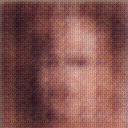
\includegraphics[width=150px]{500_fake_images/samples_5_116.png}%
\caption{A Black And White Photo Of A Black And White Cat}%
\end{figure}

%
\end{document}